\documentclass[envcountsame]{cls/cccg15}
\usepackage{graphicx}

\usepackage{amssymb,amsmath}
\usepackage[mathscr]{euscript}

\usepackage{graphicx}
\usepackage{caption,subcaption}

\usepackage[noend]{algpseudocode}


%----------------------- Environments --------------------------
\newtheorem{corollary}{Corollary} 
\newtheorem{problem}{Problem}
\newtheorem{algorithm}{Algorithm}
\newtheorem{definition}{Definition}


%------------------------ Paper Notations -----------------------------
\DeclareMathOperator*{\argmin}{arg\,min}


%-------------------------- Notations ------------------------------------
\newcommand{\cO}{\ensuremath{{\rm O}}}
\newcommand{\st}{\textsuperscript{\textit{st}} }
\newcommand{\nd}{\textsuperscript{\textit{nd}} }
\newcommand{\nth}{\textsuperscript{\textit{th}} }

\newcommand{\IN}{\ensuremath{\mathbb{N}}} 
\newcommand{\IZ}{\ensuremath{\mathbb{Z}}} 
\newcommand{\IQ}{\ensuremath{\mathbb{Q}}} 
\newcommand{\IR}{\ensuremath{\mathbb{R}}} 
\newcommand{\IC}{\ensuremath{\mathbb{C}}} 


\newcommand{\set}[1]{\left\{ #1 \right\}}
\newcommand{\seq}[1]{\left< #1 \right>}
\newcommand{\ceil}[1]{\left\lceil{#1}\right\rceil}
\newcommand{\floor}[1]{\left\lfloor{#1}\right\rfloor}
\newcommand{\card}[1]{\left|{#1}\right|}
\newcommand{\setcomp}[1]{\overline{#1}}
\newcommand{\provided}{\,:\,}

\newcommand{\poly}{\mathop{\mathrm{poly}}}
\newcommand{\polylog}{\mathop{\mathrm{\scriptsize polylog}}}
\newcommand{\lcm}{\mathop{\mathrm{lcm}}}

\newcommand{\lee}{\leqslant}
\newcommand{\gee}{\geqslant}
\renewcommand{\leq}{\lee}
\renewcommand{\le}{\lee}
\renewcommand{\geq}{\gee}
\renewcommand{\ge}{\gee}
\newcommand{\lei}{\prec}

\newcommand{\OPT}{\ensuremath{\mathop{\mathrm{OPT}}}}
\newcommand{\APX}{\ensuremath{\text{\sc APX}}}
\newcommand{\opt}{\ensuremath{\mbox{\tt opt}}}
\newcommand{\apx}{\ensuremath{\mbox{\tt apx}}}

\newcommand{\eps}{\varepsilon}
\newcommand{\bslash}{\!\setminus\!}
\newcommand{\bigOmega}{{\rm\Omega}}
\newcommand{\etal}{{\em et~al.\/}}
\newcommand{\REM}[1]{}
\newcommand{\qed}{}
\newcommand {\backspace}{\vspace{-3em}\\}

\newcommand{\linprog}[6]{
  \begin{alignat}{2}
    \text{#1}  \quad & #2\\
    \text{s.t.}  \quad & #3 & \qquad #4 \notag\\
                     & #5 & \qquad #6 \notag
  \end{alignat}}
  
\newcommand*\samethanks[1][\value{footnote}]{\footnotemark[#1]}


%----------------------- Title -----------------------------------------
\title{Streaming $2$-Center with Outliers in High Dimension}
\author{Hamid~Zarrabi-Zadeh\thanks{Department of Computer Engineering, 
	Sharif University of Technology. 
	{\tt zarrabi@sharif.edu}}
	\and 
}


%------------------------------ Text -------------------------------------
\begin{document}

\maketitle
\pagestyle{plain}

% ---------------------- Abstract --------------------------------------

\begin{abstract}

\end{abstract}

% ---------------------- Introduction ---------------------------------

\section{Introduction}





% ---------------------------- Preliminaries -------------------------------

\section{Preliminaries}
\label{sec:pre}
Let $B(c,r)$ denote a ball with center $c$ and radius $r$. We denote by $pq$ the straight line segment between these two points and by $\card{pq}$ the length of this segment. 
%kiana: tarife delta ro chanja didam nagofte budan! benazaram ma ham mitunim nagim, baz age fek mikonin lazeme tarif konam
%Behnam: be nazaram alan bashe behtare, age doctor khast hazf mikone
Define $\delta$ of two balls $B(c,r)$ and $B'(c',r')$, the minimum distance between $B$ and $B'$ which is equal to $\card{cc'}-r-r'$.

Let $B_{2,1}^*(c_{2,1}^*, r_2^*)$ and $B_{2,2}^*(c_{2,2}^*, r_2^*)$ denote the optimal solution to $2$-center problem with $z$ outliers. By $\delta^*$ we denote the distance between $B_{2,1}^*$ and $B_{2,2}^*$, that is, $\delta^* = \max (0, \card{c_1^*c_2^*} - 2r^*)$. 

Two congruent balls $B_1$ and $B_2$ with radius $r$ are said to be \emph{$C$-separated}, whenever the distance $\delta$ of two balls is at least $Cr$.

%Let $\mathcal{P}$ be a configuration of $n$ point in $d$-dimensional Euclidean space. A point $c_p$, not necessarily in $\mathcal{P}$, is a \emph{centerpoint} of $\mathcal{P}$, if no open half-space that omits $c_p$ contains more than $\frac{dn}{d+1}$ points of $\mathcal{P}$.

% kiana: man be nazaram in tarif painie vase center point behtare
% Behnam: bahat moafegham

Given an $n$-point set $\mathcal{P}$ in $d$ dimensions, a point $c \in R^d$ is called a \emph{centerpoint} of $\mathcal{P}$ if any halfspace containing $c$ contains at least $\ceil{\frac{n}{d + 1}}$ points of $\mathcal{P}$. In other words, any halfspace (or convex set) that avoids a centerpoint can contain at most $\floor{\frac{dn}{d + 1}}$ points of $\mathcal{P}$.


%-------------------------- 1-center ---------------------------------

\section{A Simple $2$-Approximation Algorithm for $1$-Center with Outliers}

\begin{algorithm}
\label{alg:1center}
\leavevmode
\begin{algorithmic}
\Function{$1$-centerWithOutliers}{$\mathcal{P}, z$}
	\State Let $p_i$ denote the elements of $\mathcal{P}$, for $i \in \set{1, \dots, n}$.
	\ForAll{$i \gets 1, \dots, z+1$}
		\State Assume $p_i$ is a non-outlier point in optimal solution.
		\State $B(c_i, r_i) \gets$ \Call{KnownPoint}{$\mathcal{P}, z, p_i$}
	\EndFor
	\State $i^* \gets \argmin_{i=1}^{z+1} r_i$
	\State \Return $B(c_{i^*}, r_{i^*})$
\EndFunction
\Statex
\Function{KnownPoint}{$\mathcal{P}, z, p$}
	\State $B \gets B(p, 0)$
	\State $Q \gets \emptyset$
	\For{$p'$ in $\mathcal{P}$}
		\If{$p' \notin B$}
			\State Insert $p'$ into $Q$
			\If{$\card{Q} = z + 1$}
				\State Remove from $Q$ a point $q$ which is closest to $p$.
				\State $B \gets B(p, \card{pq})$
			\EndIf
		\EndIf
	\EndFor
	\State \Return{B}
\EndFunction
\end{algorithmic}
\end{algorithm}
Function \textproc{KnownPoint} in Algorithm~\ref{alg:1center}, takes a point $p$ as an argument which is guaranteed to be a non-outlier point in the optimal solution. To overcome the lack of knowledge about such a point, function \textproc{$1$-centerWithOutliers} tries each of the first $z+1$ points of the stream as a candidate for a non-outlier point and generates a ball for each, using function \textproc{KnownPoint}. It returns the ball with the minimum radius. Note that, due to space limitations inherent to streaming data model, the body of for-all loop in function \textproc{$1$-centerWithOutliers} is run in parallel.

\begin{theorem}
Algorithm~\ref{alg:1center} is a $2$-approximation algorithm for $1$-center problem with $z$ outliers, in any dimension.
\end{theorem}

\begin{proof}
Let $B^*(c^*, r^*)$ be the optimal solution. Clearly, there exists a point $p$ among the first $z+1$ points of $\mathcal{P}$, which is not an outlier in the optimal solution. Since $p \in B^*$, then $\card{pp'} \le 2r^*$ for any point $p'\in B^*$. There is at least one point $q'$ among the $(z+1)$-furthest points from $p$ that is not an outlier in the optimal solution. Thus $\card{pq} \le \card{pq'} \le 2r^*$ and Algorithm~\ref{alg:1center} returns a valid solution of radius at most $2r^*$. So the proof is complete.
\end{proof}

\begin{figure}[h]
	\centering
	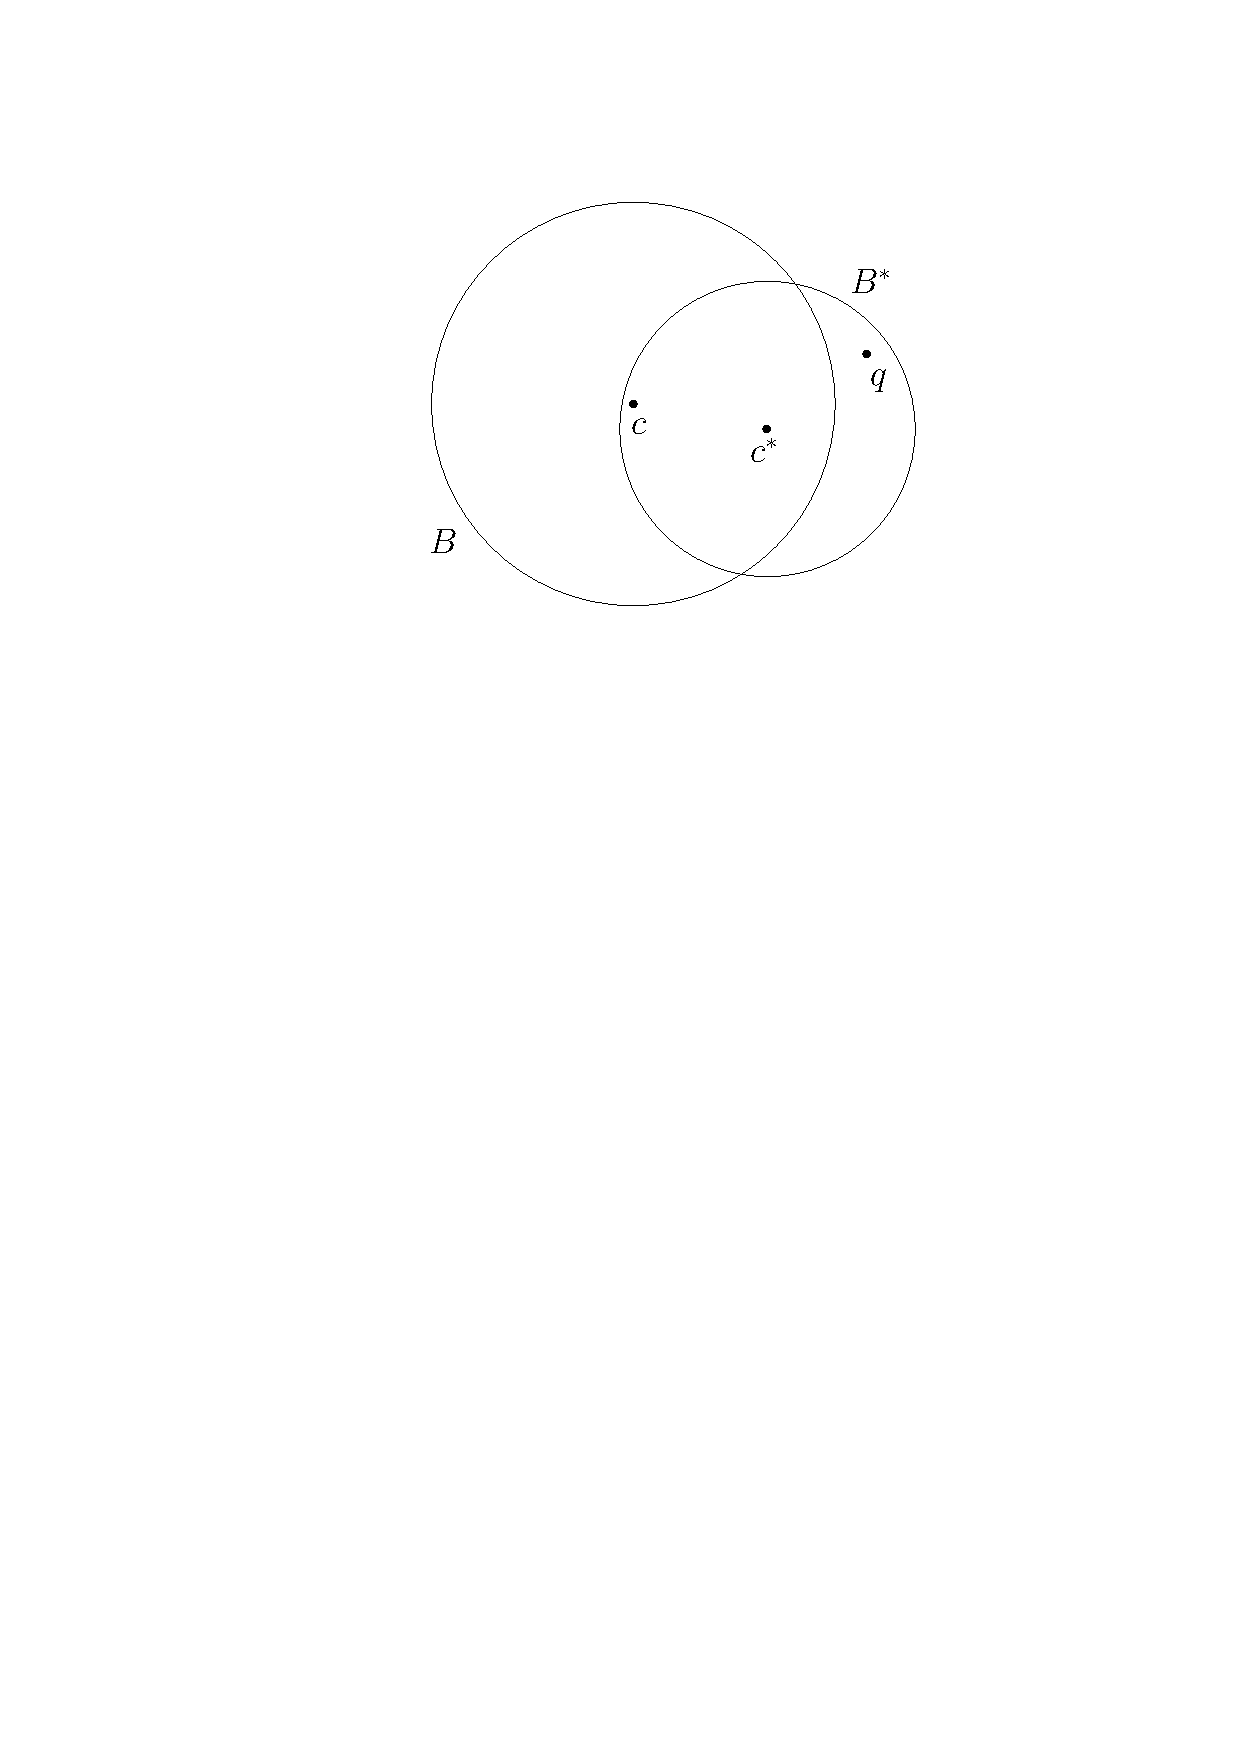
\includegraphics[width=17em]{figs/one-center}
	\caption{Output of Algorithm~\ref{alg:1center}}
	\label{fig:1center}
\end{figure}

% Behnam: Aks be nazaram gooya nist ziad. va inke jaii behesh refrence dade nashode!

The space complexity of Algorithm~\ref{alg:1center} is $\cO(z^2 + zd)$, the update time is $\cO (z \log z + zd)$ and the query time is $\cO (z)$.
If a non-outlier point $p$ is known then the space, update time and query time complexity of algorithm can be reduced by a factor of $z$.



%-------------------------- 2-center ---------------------------------

\section{The $2$-Center Problem with $z$ Outliers}

\begin{theorem}
For any fixed $d > 1$, our single-pass data stream algorithm whose working space and update time are polynomial in $d$ and sub-linear in $n$ and returns two centers that guarantees a $(1.8 + \eps)$-approximation for the Euclidean $2$-center problem with outliers.
\end{theorem}

%--- from kim and ahn

In all the algorithms given in this section it is assumed that $p_1$ is a non-outlier point. It is not hard to see that, this limitation can be remedied by considering $\cO(z)$ parallel instances of the algorithm, similar to Algorithm~\ref{alg:1center}.
% Behnam: Move this to upper section, this assumption can be used for previous algorithm

In Section \ref{subsec:smaller}, we give a description of our algorithm for a given $r' > 0$ for the case where $\delta^* < C r^*$ and $1.2r^* \le r' < (1.2 + 2\eps/3)r^*$, our algorithm returns a $(1.8 + \eps)$-approximate solution. We explain how to find such an $r'$ and present a full description of our algorithm for the case where $\delta^* < C r^*$ in Subsection~\ref{subsec:findr}. Then we inspect the case where $\delta^* \ge C r^*$ in Subsection~\ref{subsec:bigger}.


\subsection{The Case $\delta^* < C r*$}
\label{subsec:smaller}
Our idea in this section is derived from \cite[Sec.~3.1]{ahn2014computing, kim2014improved}. To avoid duplication, we just outline the important parts of their algorithm and our modifications to it. Kim's algorithm has $10$ different states. In each step one or many of the states can be valid and their algorithm considers all of them in parallel. In each state, we have two balls. A transition between the states occurs whenever a point not covered by any of the two balls has arrived in the stream. This transition graph starts with a blank node (with no balls) and has depth four (without considering the end nodes). It is straightforward to see that this transition graph is a DAG.
Our modification is on the transition part.
Points that are covered by current solution can safely be ignored, as they do not cause any transitions in the state, and only those points that lie outside the solution are candidates for being an outlier.
In each state the number of points that should be considered as outlier is unknown. So all the possible choices should be considered. It is sufficient to have four integers, $n_1,\dots, n_4$ representing the number of outliers in depth $1$ to $4$, such that $\sum_{i=1}^{4} n_i=z$. To sum up, the modified algorithm is defined as follows:
\begin{algorithm}
\label{alg:smallc}
\leavevmode
\begin{algorithmic}
\Function{Known$r'$}{$\mathcal{P}, z, r'$}
	\For{$(n_1, \dots, n_4) \gets \set{(n_1, \dots, n_4) \provided \sum n_i=z}$}
		\State $CS \gets B(p_1,r')$.
		\State $p_{o_2} \gets $ \Call{NthOutlier}{$n_1 + 1$}
		\If{$p_{o_2}$ arrives}
			\State $CS\gets$ the sub-case of $p_{o_2} \in B_{2, 1}^*$ $\cup$ the sub-case of $p_{o_2} \in B_{2,2}^*$.
			\For{each case $S$}
				\State $p_{o_3} \gets$ \Call{NthOutlier}{$n_2 + 1$}
				\If{$p_{o_3}$ arrives} 
					\State $CS\gets CS\setminus S$ $\cup$ the sub-case of $p_{o_3} \in B_{2, 1}^*$ $\cup$ the sub-case of $p_{o_3} \in B_{2,2}^*$.
					\For {each sub-case $S'$} 
						\State $p_{o_4} \gets$ \Call{NthOutlier}{$n_3 + 1$}
						\If {$p_{o_4}$ arrives} 
							\State Replace $S'$ with a new candidate solution.
							\State $p_{o_5} \gets$ \Call{NthOutlier}{$n_4 + 1$}
							\If{$p_{o_5}$ arrives}
								\State Abandon the solution.
							\EndIf
						\EndIf
					\EndFor
				\EndIf
			\EndFor

		\EndIf
		\State $\mathop{Sol}_{n_1,n_2,n_3,n_4} \gets$ the solution with the smallest larger radius, among all the sub-cases.
	\EndFor
	\State \Return the solution $\mathop{Sol}_{n_1,n_2,n_3,n_4}$ with the smallest radius, for all valid values of $(n_1,n_2,n_3,n_4)$.
\EndFunction
\end{algorithmic}
\end{algorithm}
Here, \textproc{NthOutlier}$(n)$ returns the $n$\nth next point in $\mathcal{P}$ that does not lie in current candidate solution.

\begin{theorem}
Given $\delta^* < C r*$ and $1.2r^* \le r' < (1.2 + 2\eps/3)r^*$, Algorithm~\ref{alg:smallc} uses $\cO (dz^3)$ space and returns a $(1.8+\eps)$-approximate solution. Algorithm~\ref{alg:smallc} spends $\cO (dz^3)$ update time for each point in $\mathcal{P}$ and answers a query in $\cO (dz^3)$.
\end{theorem}

\begin{proof}
Since our algorithm considers all possible input cases of streaming points, there is at least one feasible solution. Since every feasible solution has its larger radius at most $3r'/2$, the final solution has larger radius at most $3r'/2 \le (1.8 + \eps)r^*$.
For space complexity, our algorithm maintains at most two balls in each case, and therefore it uses $\cO(dz^3)$ space. Whenever the next point is inserted, the algorithm updates the solution for each sub-case in $\cO (d)$ time. Therefore, the algorithm spends $\cO (dz^3)$ update time for each point of $\mathcal{P}$. Answering a query consists of choosing the minimum radius among all the candidate solutions, which amounts to $\cO (dz^3)$ time.
\end{proof}


\subsubsection{Finding $r'$}
\label{subsec:findr}

\begin{lemma}
\label{lem:1lt2}
A $1$-center optimal solution with $z$ outliers for a streaming set of points is also an upper bound for the $2$-center optimal solution with $z$ outliers.
\end{lemma}
\begin{proof}
Let $B^*(c^*, r_1^*)$ be the optimal solution for the $1$-center problem. Let $B'$ be a ball with radius $r_1^*$ and center at $\infty$. Clearly, $(B^*, B')$ is a solution for $2$-center problem. Thus, the proof is complete.
\end{proof}

\begin{lemma}
\label{lem:2lt1}
Let $r_1^*, r_2^*$ be the radius of $1$-center and $2$-center optimal solutions with $z$ outliers, respectively. Then $r_1^* < \left(\frac{C}{2} + 2\right) r_2^*$.
\end{lemma}
\begin{proof}
Suppose that $(B_{2, 1}^*(c_1^*, r_2^*), B_{2,2}^*(c_2^*, r_2^*))$ is an optimal solution for $2$-center problem. Consider $m$ as the midpoint of segment 
$c_1^*c_2^*$.
Clearly, $B\left(m, \frac{\delta}{2} + 2r_2^*\right)$ covers both $B_{2, 1}^*$ and $B_{2,2}^*$. So it is a solution for $1$-center problem and the proof is complete.
\end{proof}

\begin{figure}[h]
	\centering
	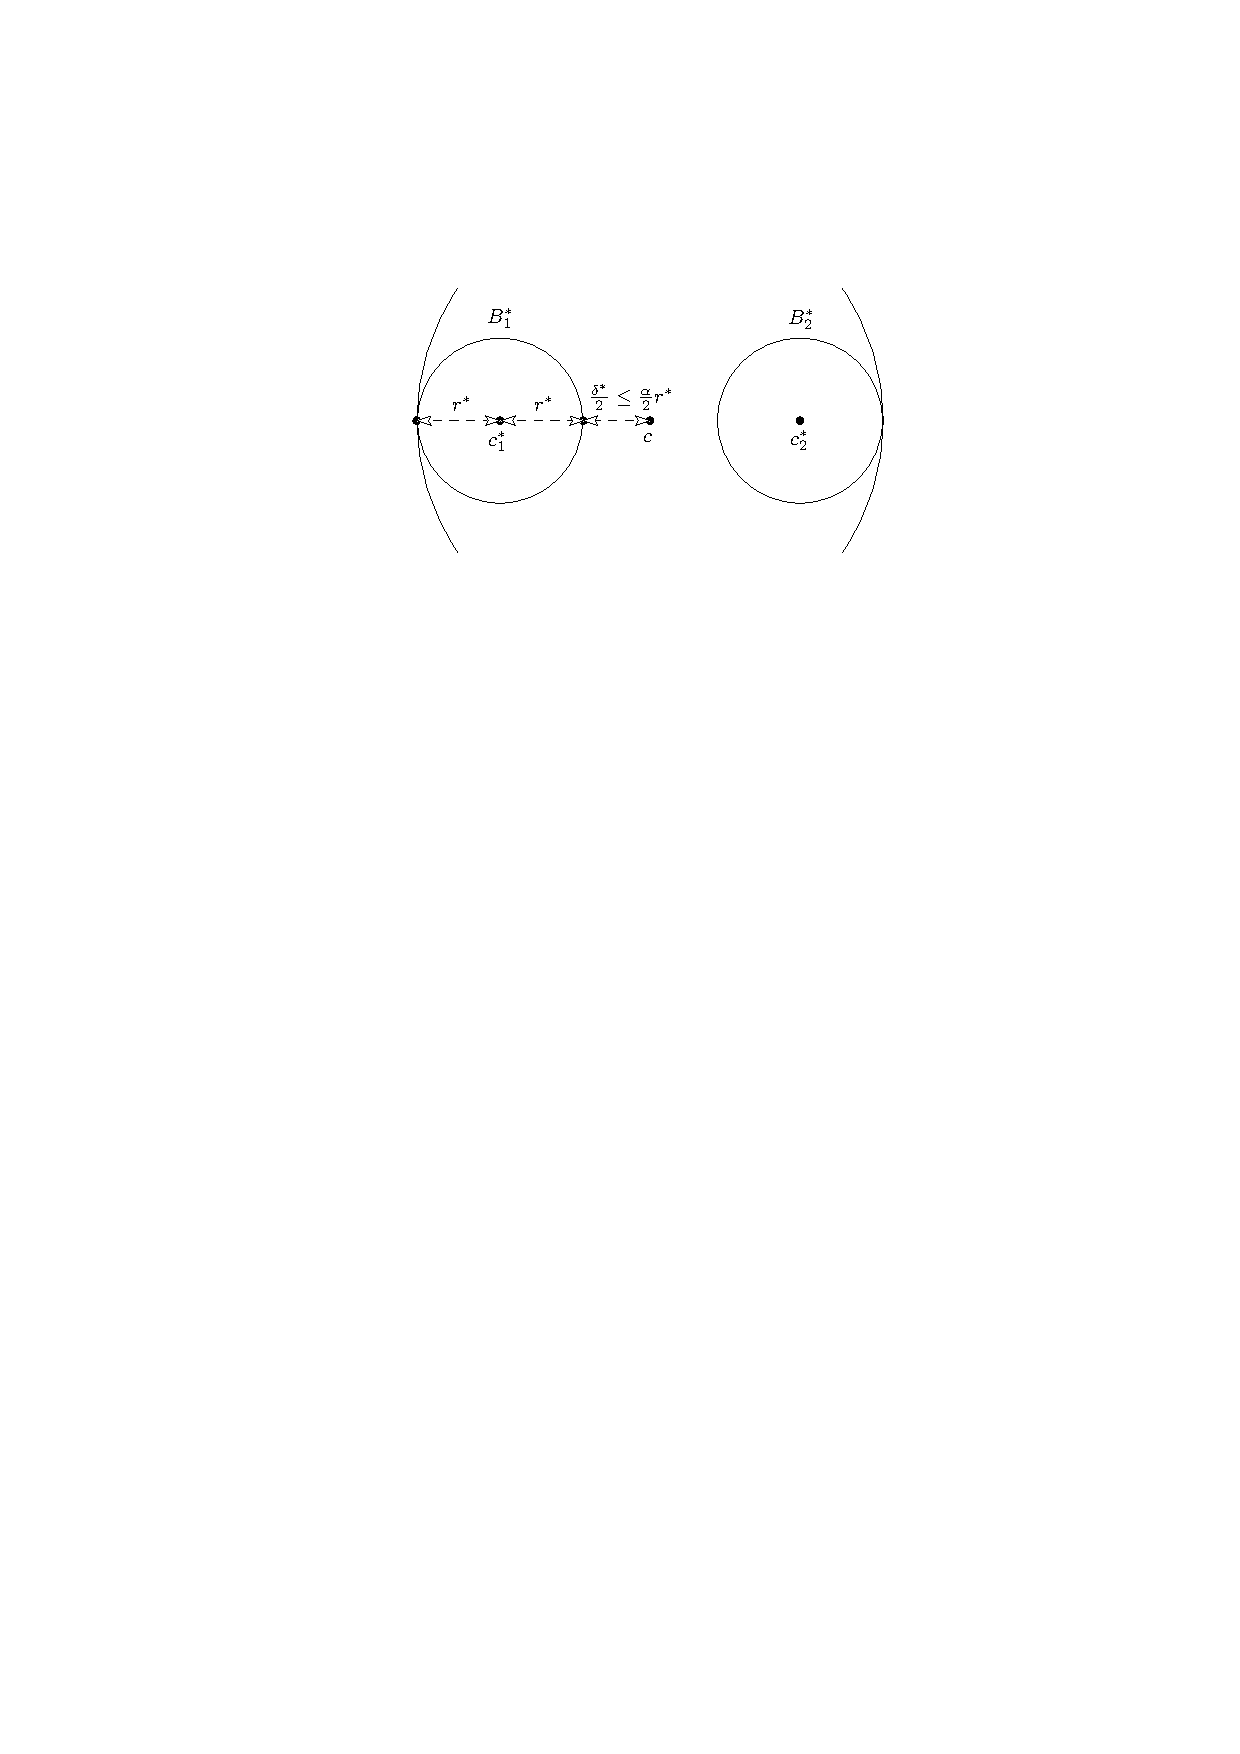
\includegraphics[width=19em]{figs/2lt1}
	\caption{Proof of Lemma~\ref{lem:2lt1}}
	\label{fig:2lt1}
\end{figure}

Algorithm~\ref{alg:1center} finds a $2$-approximation for $r_1^*$. By Lemma \ref{lem:1lt2} and \ref{lem:2lt1}, it gives a $2\left(\frac{C}{2} + 2\right)$-approximation for $r_2^*$.

\begin{obs}
\label{obs:2apr}
Let $r_1$ and $k_0$ be two positive real numbers. Define $k=k_0 2^i$ to be the smallest real number satisfying the inequality $k \ge r_1$, where $i$ is a non-negative integer. Clearly, $k$ is a $2$-approximation for $r_1$.
\end{obs}

%In this section, we explain how we get r' such that 1.2r^*  r' < (1.2 + 2\eps/3)r^*. The basic procedure works as follows: 

Our algorithm maintains $m=\ceil{\frac{1.2(3C+12)}{\eps}}$ candidate lengths.
For each candidate length $t$, we assume that $r' = t$ and use it to run Algorithm~\ref{alg:smallc}. We use Algorithm~\ref{alg:1center} to estimate $r'$. Let $k_i$ be the $i$\nth non-zero radius calculated by the algorithm. Obviously, the sequence of answers given by the algorithm is increasing.

Let $l_1=k_1$ and $l_i=2^j l_1$, where $l_i$ is the smallest number satisfying $l_i \ge k_i$. By Observation~\ref{obs:2apr}, $l_i$ is a $(2C + 8)$-approximation for $r_2^*$. If we divide the interval $(0, 1.2 l_i]$ into $m$ equal segments, then length of each segment is at most $2/3 \eps r_2^*$ and the endpoints as candidates are $\mathcal{L}_i = \set{j \times t_i \provided j = 1, \dots, m}$ where $t_i = \frac{1.2 l_i}{m}$. 
The inequality $1.2 r_2^* \le j \times l_i \le (1.2 + \frac{2\eps}{3})r_2^*$ holds for at least one of these candidates.

\begin{figure}[h]
	\centering
	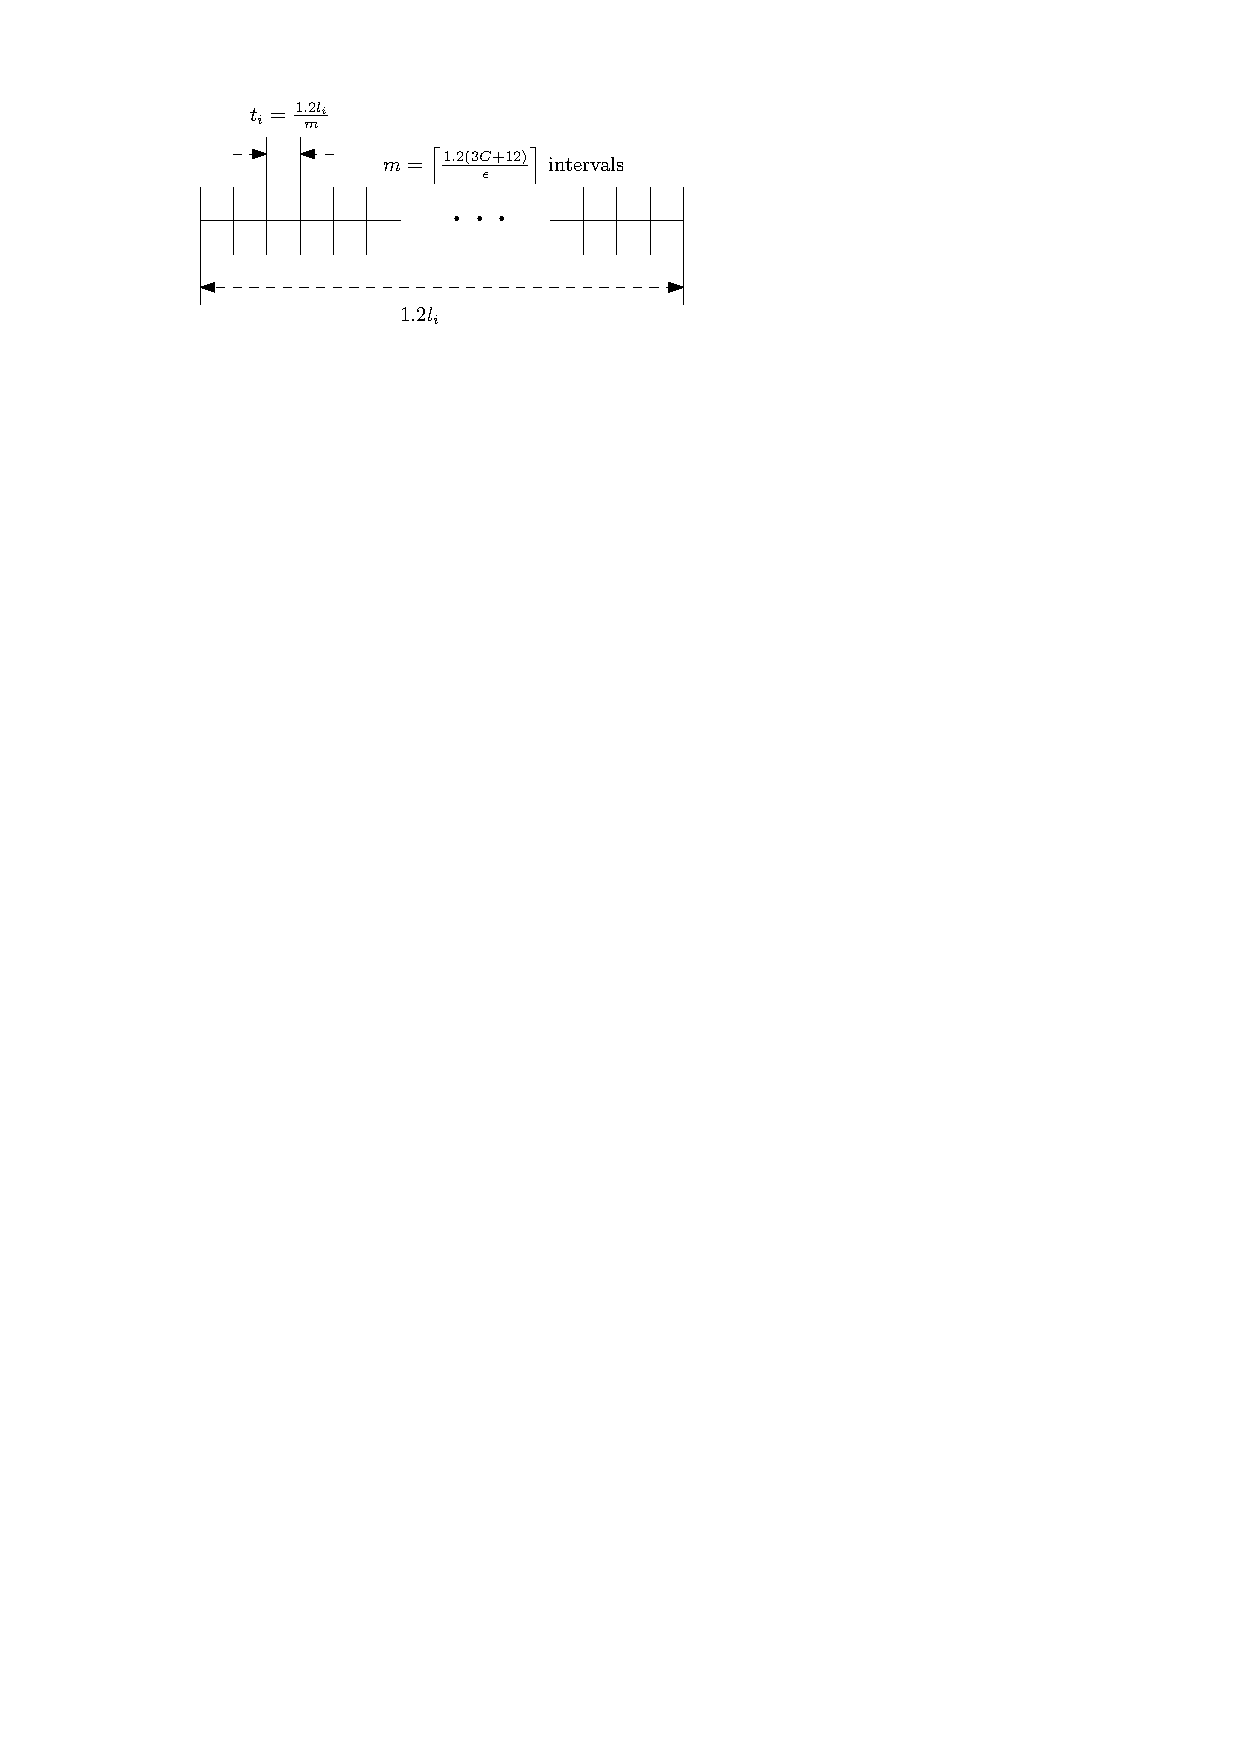
\includegraphics[width=21em]{figs/findr}
	\caption{Subdivision of $(0, 1.2 l_i]$ interval}
	\label{fig:findr}
\end{figure}

%kiana: bacheha in paragraph paini kheili bad bud benazaram. man ye talashai rush kardam vali hanuzam benazaram jaye kar dare
%Behnam: khoobe
When the first non-zero radius is observed, $l_1$ is set. Algorithm~\ref{alg:smallc} should be executed for each candidate in $\mathcal{L}_1$ for all the previous points, which have been stored in a buffer. It is not hard to see that the space complexity for storing these points is $\cO(z)$. For each new point, if $l_i=l_{i-1}$ then $\mathcal{L}_i = \mathcal{L}_{i-1}$ and it suffices to add the new point to all parallel instances corresponding to candidates in $\mathcal{L}_i$. Otherwise, Algorithm~\ref{alg:smallc} should be executed for all of the candidates in $\mathcal{L}_i$, with all the points. But this is not achievable due to space limitations. To remedy
%kiana, sahand: remedy?? really??
this problem, note that if the candidate $x_j=j \times t_i \in \mathcal{L}_i$ is also in $\mathcal{L}_{i-1}$, there is no need to start Algorithm~\ref{alg:smallc} over and the current execution will be continued. If $x_j \notin \mathcal{L}_{i-1}$, then it is certain that $x_j \ge l_{i - 1}$ (Observe that $l_i=ul_{i-1}$, for some $u\in \mathbb{N}$). Since the ball $B_1(p_1, l_{i-1})$, obtained from Algorithm~\ref{alg:1center}, has at most $z$ outliers, all the non-outlier points lie in the candidate balls in Algorithm~\ref{alg:smallc}.
%kiana: in jomle balai oke be nazaretun? 
% Behnam: be nazare man gheire vazehe, be nazaram baiad begim hade aksar z ta biroonan, oonam oonaii ke too buffer algorithme 1 an
These outliers have been stored in a buffer, so for the new candidate length, it suffices to execute Algorithm~\ref{alg:smallc} with only the outlier points of $B_1$.

\begin{theorem}
\label{thm:1st-cmplx}
Algorithm~\ref{alg:smallc} uses $\cO(\frac{dz^3}{\eps})$ space, and takes $\cO(\frac{dz^4}{\eps})$ and $\cO(\frac{dz^3}{\eps})$ time for update and query, respectively.
\end{theorem}

\subsection{The Case $\delta^* \ge C r^*$}
\label{subsec:bigger}


\begin{obs}
\label{obs:c+4}
Let $d$ be the distance between arbitrary pair of points from two $C$-separated balls. Then $1 \le \frac{d}{\delta} \le \frac{C+4}{C}$.
\end{obs}

\begin{figure}[h]
	\centering
	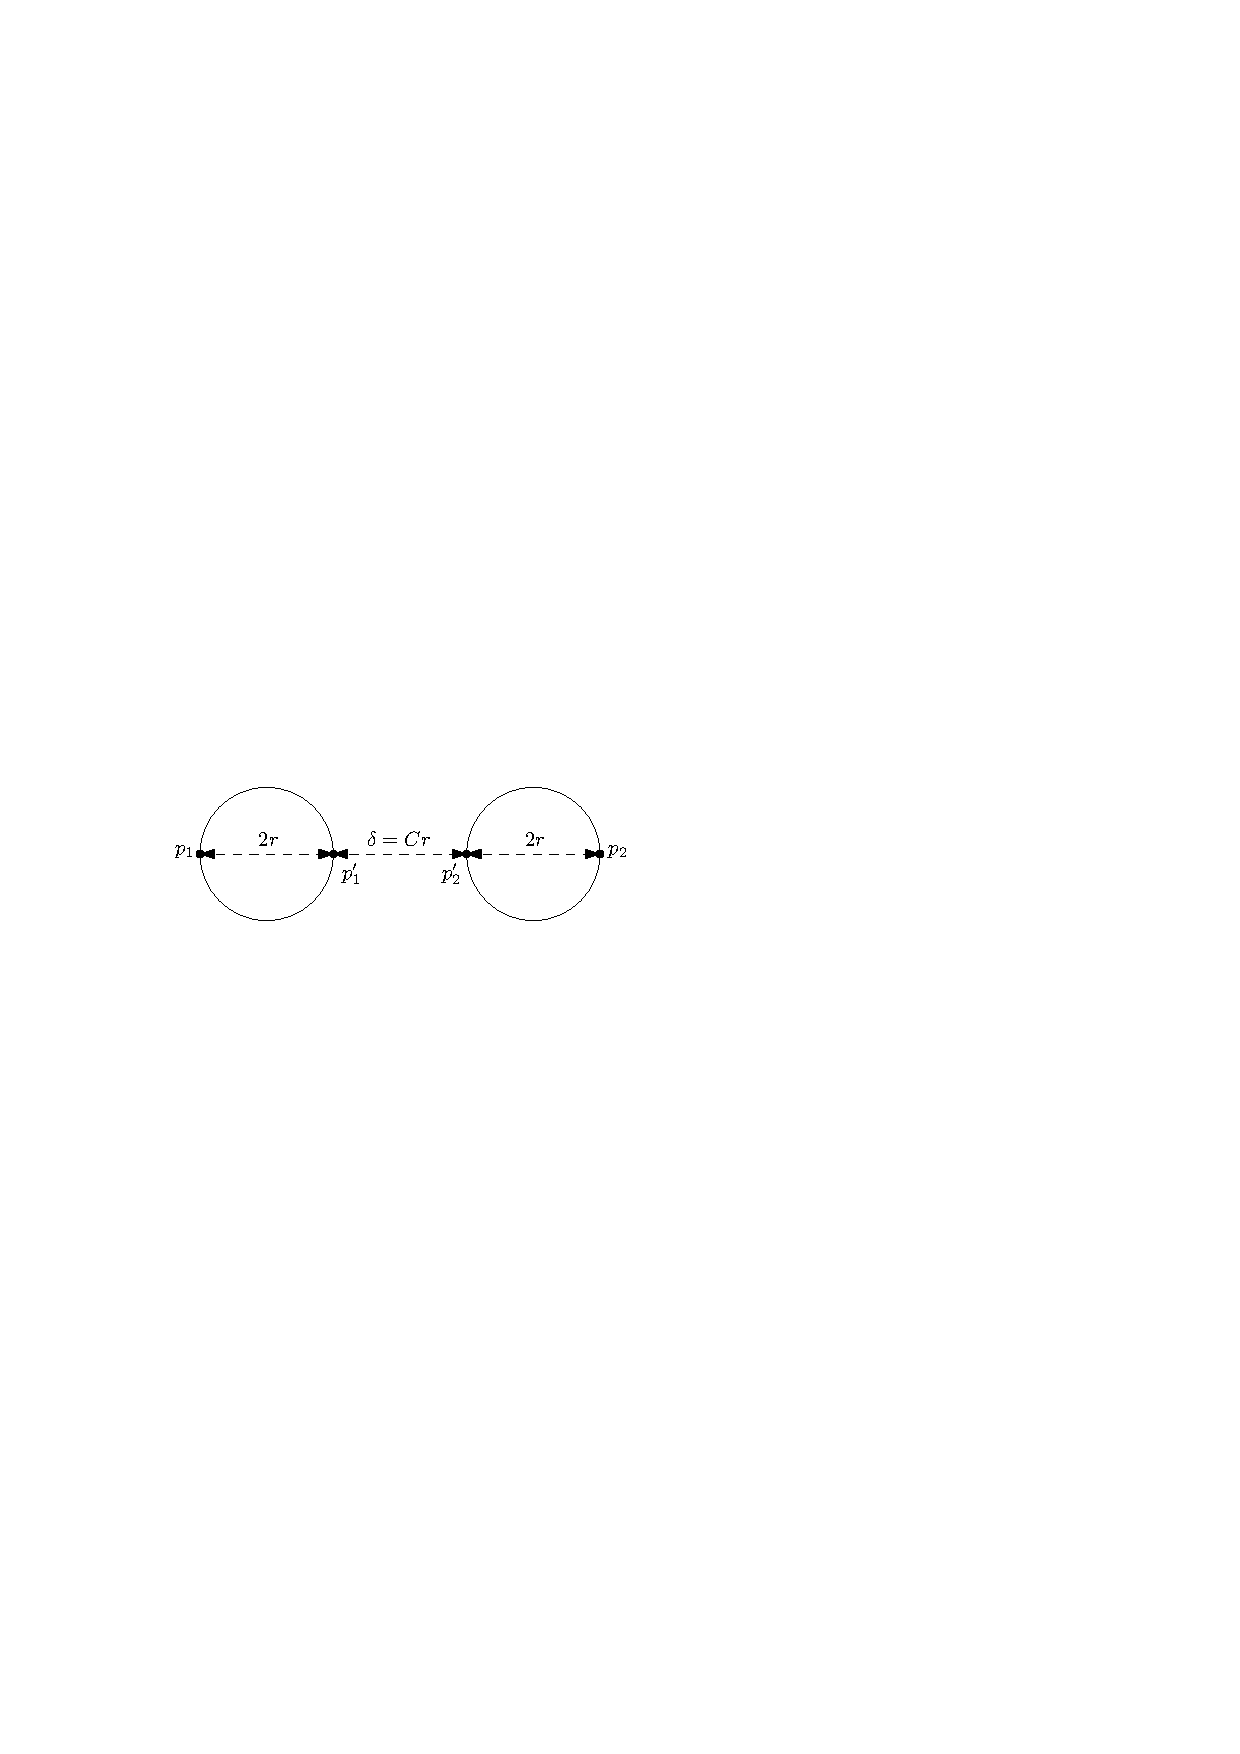
\includegraphics[width=21em]{figs/c_plus_4}
	\caption{Depiction of two extreme case of Observation~\ref{obs:c+4}}
	\label{fig:c+4}
\end{figure}

\begin{obs}
\label{obs:intersection}
Let $B_1$ and $B_2$ be two disjoint balls with distance $\delta$ and $B$ be an arbitrary ball of radius at most $\frac{\delta}{2}$. Then $B$ can intersect at most one of $B_1$ and $B_2$.
\end{obs}

\begin{lemma}
\label{lem:c-sep}
Let $\mathcal{P}$ be a set of points and assume that $B_{2,1}^*$ and $B_{2,2}^*$ are $C$-separated ($C \ge 4$) and let $p_1$ be an arbitrary point in $B_{2,1}^*$. Define $S$ as the $z+1$ furthest points of $\mathcal{P}$ from $p_1$. Then $S \cap B_{2,2}^*$ is nonempty.
\end{lemma}
\begin{proof}
By contradiction, assume that $S \cap B_{2,2}^*$ is empty. It is clear that $S$ contains at least one non-outlier point. Let $q$ be the furthest point of $S \cap B_{2,1}^*$ from $p_1$. Consider $B(p_1, \card{p_1q})$. It is clear that $B$ covers $\mathcal{P} \setminus S$. Since $p_1, q \in B_{2,1}^*$, then $\card{p_1q}$ is at most $2r_2^*$. Thus by Observation~\ref{obs:intersection}, $B_{2,2}^* \cap B = \emptyset$. Therefore $B_{2,2}^* \cap \mathcal{P} = \emptyset$ and hence $B_{2,2}^*$ is empty, which contradicts the optimality of this solution.
\end{proof}

Let $B_1, B_2$ and $B_u$, be instances of a data structure that supports adding a point and gives a $\beta$-approximation for $1$-center problem with $k$ outliers, for $k=0,\dots,z$ (This data structure, does not need to maintain all the points. Suppose that it has a buffer with length $(d+1)(z+1)$ that maintains the most recently added points). Algorithm~\ref{alg:case2} assumes point $p_1$ to be in $B_{2,1}^*$. This algorithm maintains $c_1$ as an arbitrary point in $B_{2,1}^*$ and $c_2$ as a candidate that may be in $B_{2,2}^*$. It tries to divide points into three subdivisions:
\begin{itemize}
\item $B_1$, a subset of $\mathcal{P}$ where $B_1 \cap B_{2,2}^* = \emptyset$, that is a set of points that provably lie outside $B_{2, 2}^*$.
\item $B_2$, a subset of $\mathcal{P}$ along with a \emph{candidate point} $c_p$, such that if $B_{2, 2}^*$ covered the candidate point, then $B_2 \cap B_{2, 1}^* = \emptyset$.
\item Buffer, with size at most $z$ that if $c_p \in B_{2, 2}^*$ then all of them are outliers.
\end{itemize}
Algorithm~\ref{alg:case2} also maintains $B_u$ as union of $B_1$ and $B_2$.

%\begin{algorithmic}
%\Procedure{add to furthest buffer(z+1)}{p}
%	\State add p to buffer
%	\If{size of buffer $> z+1$}
%		\State remove nearest point from $p_1$
%	\EndIf
%\EndProcedure
%\end{algorithmic}

\begin{lemma}
\label{lem:(z+1)-furthest}
Let $p_1$ be an arbitrary points in $B_{2,1}^{*}$ and $q$ be the $(z+1)$\st furthest point from $p_1$. Then $\frac{C}{C+4}\card{qp_1}$ is a lower bound for $\delta^*$.
\end{lemma}
\begin{proof}
Due to Lemma~\ref{lem:c-sep}, there exists $p_2 \in B_{2,2}^*$ such that $\card{p_1p_2} \ge \card{qp_1}$. Thus, by Observation~\ref{obs:c+4}, $\frac{C}{C+4} \card{p_1p_2} \le \delta^*$. The claim follows immediately.
\end{proof}

Function \textproc{AddTo$B_1$} is used to add a point $p$ to $B_1$. The point will be added only if the point is within $\delta$-radius of the center $c_1$, where $\delta$, calculated by Algorithm~\ref{alg:case2}, is $\frac{C}{C+4}\card{qc_1}$ and $q$ is the $(z+1)$\nth furthest point from $c_1$. By Lemma~\ref{lem:(z+1)-furthest}, $\delta$ is a lower bound for $\delta^*$. So any point within $\delta$-radius of $c_1$ is guaranteed to lie outside $B_{2,2}^*$. Thus Function \textsc{AddTo$B_1$} does not violate the property $B_1 \cap B_{2,2}^* = \emptyset$.
\begin{algorithmic}
\Function{AddTo$B_1$}{$p$}
	\If{$p \in B(p_1, \delta)$}
		\State $B_1 = B_1 \cup \set{p}, B_u = B_u \cup \set{p}$
		\State \Return{true}
	\Else
		\State \Return{false}
	\EndIf
\EndFunction
\end{algorithmic}

Function \textproc{AddTo$B_2$} is used to add a point $p$ to $B_2$. Initially, $B_2$ is empty and $c_2$ and $r_c$ are not initialized. When an appropriate candidate is found, Algorithm~\ref{alg:case2} sets $c_2$ to that candidate and $r_c$ to $\frac{2\card{c_1c_2}}{C}$ and thereafter
%kiana: bacheha kudumetun in kalame ro gozashtin? azash motmaeni? man hichja nadide budamesh
points are added to $B_2$ only if they lie within $r_c$-radius of $c_2$. At this point $c_2$ is considered as the \emph{candidate point} $c_p$. Clearly the subdivision property for $B_2$ holds initially when $B_2$ consists of the single point $c_2$. All the subsequent points added to $B_2$ are within $r_c$-radius of $c_2$ and given $C\ge 7$, by Observation~\ref{obs:intersection} subdivision property is invariant under this operation.

When $\card{B_2}$ reaches $(d+1)(z+1)$, we move \emph{candidate point} to center point of $B_2$ and $r_c$ is increased by a factor of $(2 + \frac{2}{C})$ to completly cover the new \emph{candidate point} and it's surronding ball. It is easy to see that $(2 + \frac{2}{C})r_c < \frac{\delta}{2}$ provided $C \ge 14$ and thus by Observation~\ref{obs:intersection} the property is not violated.

\begin{algorithmic}
\Function{AddTo$B_2$}{p}
	\If{$c_2$ is set and $p \in B(c_2, r_c)$}
		\State $B_2 \gets B_2 \cup \set{p}, B_u \gets B_u \cup \set{p}$
		\If{$\card{B_2} = (d+1)(z+1)$}
			\State $r_c \gets  (2 + \frac{2}{C}) \times r_c$
			\For{$p$ in Buffer}
				\If{$p$ in $B(c_2, r_c)$}
					\State $B_2 \gets B_2 \cup \set{p}, B_u \gets B_u \cup \set{p}$
				\EndIf
			\EndFor
		\EndIf
		\State \Return{true}
	\Else
		\State \Return{false}
	\EndIf
\EndFunction
\end{algorithmic}



\begin{prop}
Any set $\mathcal{P}$ of points in $d$-dimensional Euclidean space has a centerpoint.\cite{edelsbrunner}
\end{prop}

\begin{cor}
\label{cor:omitting-centerpoint}
Given a set $\mathcal{P}$ of $k(d+1)$ points in $d$-dimensional Euclidean space, there is a point $c_p$, not necessarily in $\mathcal{P}$, that any convex object that does not cover $c_p$, leaves at least $k$ points of $\mathcal{P}$ uncovered.
\end{cor}

Let new \emph{candidate point} be $c_p$, centerpoint of points in $B_2$, when $(z+1)(d+1)$ points have been added to $B_2$. We claim that with $B_2 = B(c_2, (2 + \frac{2}{C})r_c)$, ball $B(c_p, \frac{2\card{c_1c_p}}{C})$ completly covered.
If $c_p \in B_{2,2}^*$ then by Observation~\ref{obs:c+4}, $r^* \le \frac{\card{c_1c_p}}{C}$. Thus $B_{2,2}^* \subseteq B(c_p, \frac{2\card{c_1c_p}}{C})$.
Since:
\[
\frac{2\card{c_1c_p}}{C} \leq \frac{2}{C}(\card{c_1c_2} + r_c) \leq (1 + \frac{2}{C})r_c
\]
 then $B_{2,2}^* \subseteq B(c_p, (1 + \frac{2}{C})r_c) \subseteq B(c_2, (2 + \frac{2}{C})r_c)$. Thus supposing $C \ge 14$ and by Observation~\ref{obs:intersection}, $B_2 \cap B_{2,1}^* = \emptyset$. Thus the claim follows.

At some point during the execution of Algorithm \ref{alg:case2}, the assumption about $c_p \in B_{2,2}^*$ might be contradicted when the buffer overflows. We can then conclude that $c_2 \notin B_{2,2}^*$.
At this point, behavior of Algorithm~\ref{alg:case2} depends on size of $B_2$ relative to $(d+1)(z+1)$:
\begin{itemize}
\item If $\card{B_2} < (d+1)(z+1)$ then $c_2$ can be added to $B_1$, by definition of $B_1$.
The algorithm then tries all points in $B_2 \cup \mbox{Buffer} \setminus \set{c_2}$, until it finds a suitable candidate point for $c_2$ that does not leave too many points uncovered. Note that at most $(z+1)(d+1) + z$ points have to be tried.
\item If $\card{B_2} \ge (d+1)(z+1)$, let $q$ be the $(z+1)$\st furthest point from $p_1$ and $p'$ be the nearest point of ball $B_2(c_2, r_c)$ to $p_1$. Then $\card{qp_1} > \card{p'p_1}$, since $B_2$ contains more than $z+1$ points. So by Lemma~\ref{lem:(z+1)-furthest}:
\[
\delta \ge \frac{C \card{qp_1}}{C+4} \ge \frac{C}{C+4} (\card{c_1c_2} - r_c) = \frac{C^2 - 2C}{2C + 8} r_c
\]
As a result, if $C \geq 14$ then $(2 + \frac{2}{C}) r_c < \frac{\delta}{2}$. As shown in Observation~\ref{obs:intersection}, the ball $B_2(c_2, (2 + \frac{2}{C}) r_c)$ has nonempty intersection with exactly one of $B_{2, 1}^*$ and $B_{2, 2}^*$ (not all of its points can be outliers). Since the buffer overflowed, the assumption about the candidate point, $c_p$, being in $B_{2,2}^*$ must have been invalid. By Corollary~\ref{cor:omitting-centerpoint} if $c_p$ is not covered, then circle $B_{2,1}^*$ leaves at least $z+1$ points of $B_2$ uncovered, and there will be more than $z$ outliers. Thus, $c_p$ has to be covered. As a result, $c_p \in B_{2, 1}^*$ and all the points of $B_2$ can be added to $B_1$. This is done by replacing $B_1$ with $B_u$ and initializing $B_2$ over again.
\end{itemize}

\begin{algorithm}
\label{alg:case2}
\leavevmode
\begin{algorithmic}
\State $\delta \gets 0, r_c \gets 0$
\State $c_1 \gets p_1$
\For{$p \in P$}
	\If{at least $z+1$ points have been processed}
		\State $q \gets$  $(z+1)$-furthest point from $c_1$
	\Else
		\State $q \gets c_1$
	\EndIf
	\State $\delta \gets \frac{C}{C+4} \card{c_1q}$
	\If{!\Call{AddTo$B_1$}{$p$} and !\Call{AddTo$B_2$}{$p$}}
		\State add $p$ to Buffer
		\While{$\card{\mbox{Buffer}} > z$}
			\If{$\card{B_2} \ge (d+1)(z+1)$}
				\State $B_1 \gets B_u$, $B_2 \gets \emptyset$
			\ElsIf{$c_2$ is set}
				\State $B_1 \gets B_1 \cup \set{c_2}$, $B_u \gets B_u \cup \set{c_2}$
			\EndIf
			\State $T \gets \mbox{Buffer} \cup B_2 - \set{c_2}$
			\State $\mbox{Buffer} \gets \emptyset, B_2 \gets \emptyset$
			\If{first iteration of while}
				\For{$p \in T$}
					\If{\Call{AddTo$B_1$}{$p$}}
						\State remove $p$ from $T$
					\EndIf
				\EndFor
			\EndIf
			\State $c_2 \gets$ arbitrary point in $T$
			\State $r_c \gets \frac{2}{C}\card{c_1 c_2}$
			\For{$p \in T$}
				\State \Call{AddTo$B_2$}{$p$}
			\EndFor				
			\State $\mbox{Buffer} \gets T \setminus B_2$
		\EndWhile
	\EndIf
\EndFor
\end{algorithmic}
\end{algorithm}

Let $B_1'$, $B_2'$ and $B_u'$ be the $1$-centers obtained from $B_1$, $B_2$ and $B_u$ by the $\beta$-approximation algorithm, respectively. To answer a query, we use these balls. By the initial assumption about $p_1$, $B_1$ contains $B_{2,1}^*$ and $B_1'$ is a $\beta$-approximation for $B_{2,1}^*$. But for $B_2$ it may be the case that our assumption about the \emph{candidate point} was incorrect or non-optimal, so $B_2'$ is not a good approximation for $B_{2,2}^*$. There are two cases for $\card{B_2}$ to be considered. If $\card{B_2} < (z+1)(d+1)$, then we can try each point in $B_2 \cup \mbox{Buffer}$ as a candidate for the \emph{candidate point}. If $\card{B_2} \ge (d+1)(z+1)$, then there is no need for points in $B_2$ to be considered, since for those points as \emph{candidate point}, $B_1$ would be replaced by $B_u$ and $B_2$ would be empty. Thus it suffices to consider points of Buffer as candidates and compare them to the solution $(B_u, \emptyset)$.

\begin{algorithm}
\label{alg:query}
\leavevmode
\begin{algorithmic}
\Function{Query}{}
	\State solutions = [\Call{QuerySubdivision}{$B_1$ $B_2$ Buffer}]
	
	\If {$\card{B_2} \geq (d+1)(z+1)$}
		\State candidates $\gets$ Buffer
	\Else
		\State candidates $\gets$ Buffer $\cup B_2 - \set{c_2}$
	\EndIf

	\For{$c_2 \in$ candidates}
		\State $r_c \gets \frac{2}{C} \card{c_1 c_2}$
		\State $B_2 \gets \emptyset$, Buffer $\gets \emptyset$ 
		\For{$p \in$ candidates}
			\If{not \Call{AddTo$B_2$}{$p$}}
				\State add $p$ to Buffer
			\EndIf
		\EndFor
		\State add \Call{QuerySubdivision}{$B_1$, $B_2$, Buffer} to solutions
	\EndFor
	\State \Return \Call{$\min$}{solutions}
\EndFunction
\Statex
\Function{QuerySubdivision}{$B_1$, $B_2$, Buffer}
	\State solutions $\gets$ empty list
	\For{$k \gets 0, \dots,(z - \card{\mbox{Buffer}})$}
		\State $r \gets \max(1-\mbox{center}(B_1, k), 1-\mbox{center}(B_2, z - \card{\mbox{Buffer}} - k))$
		\State add $r$ to solutions
	\EndFor
	\State \Return \Call{$\min$}{solutions}
\EndFunction
\end{algorithmic}
\end{algorithm}


Suppose that our data structure for maintaining $B_1$, $B_2$ and $B_u$ uses $S(n,z,d)$ space, $T(n,z,d)$ update and $Q(n,z,d)$ query time. Note that by $Q_{o}(zd,z,d)$ we mean the query time for the offline $1$-center problem with $z$ outlier in $d$ dimensions. The best known algorithm for $1$-center without outliers is $1.22$-approximation by \cite{chan2014streaming, agarwal2010streaming}. The buffering framework introduced in \cite{zarrabi2009streaming} can use this algorithm to achieve a $(1.22\sqrt{2})$-approximation ($1.22\sqrt{2} < 1.8$) for $1$-center problem with outliers.

\begin{theorem}
\label{thm:2nd-cmplx}
Space complexity of Algorithm~\ref{alg:case2} is $\cO(dz+S(n,z,d))$. It takes $\cO^*(dzT(n,z,d))$ time for update. Query time in Algorithm~\ref{alg:query} is $\cO(zQ(n,z,d) + dz(dz+zQ_o(zd,z,d)))$ and it returns two centers that guarantee a $(1.8 + \eps)$-approximation for $2$-center problem with outliers.
\end{theorem}

\begin{proof}
The space complexity for this algorithm is derived from the space used by $B_1$, $B_2$, $B_u$ and the Buffer which is obviously $\cO(dz+S(n,z,d))$. The while loop runs at most once for each point, so amortized time is $\cO(zdT(n,z,d))$. The candidates in the Algorithm \ref{alg:query} are at most $zd$ points  so the query time will easily follows.
\end{proof}

\begin{theorem}
Our algorithm uses $\cO(zS(n, z, d) + \frac{dz^4}{\eps})$ space and has time complexity $\cO^*(dz^2T(n,z,d) + \frac{dz^5}{\eps})$ and $\cO(z^2Q(n,z,d) + dz^2(dz+zQ_o(zd,z,d)) + \frac{dz^4}{\eps})$ for update and query operations, respectively. It returns a $(1.8 + \eps)$-approximate solution for $2$-center problem with outliers in any dimension.
\end{theorem}
\begin{proof}
Result follows immediately from Theorems~\ref{thm:1st-cmplx} and \ref{thm:2nd-cmplx} and the fact that $p_1$ was assumed to be a non-outlier.
\end{proof}

%--------------- BIBS --------------------

\small
\baselineskip=.85\baselineskip
\bibliographystyle{abbrv}
\bibliography{bibs/abbrv,bibs/ref}


\end{document}

